\documentclass[a4paper]{article}

\usepackage[utf8]{inputenc}
\usepackage{graphicx}
\usepackage{float}
\usepackage[caption = false]{subfig}
\usepackage{amsmath}
\usepackage{indentfirst}
\usepackage{hyperref}
\usepackage[margin=2.8cm]{geometry}
\usepackage{ragged2e}
\usepackage{makecell}

\title{Clustering Molecular Structures for Next-generation Solar Cell Material Discovery}
\author{Gustave Li}
\date{August 24, 2021}

\begin{document}

\maketitle

\section{Abstract}

\section{Introduction}
The Carotenoid-Porphyrin-\(\text{C}_{60}\) (\(\text{CPC}_{60}\)) triad molecule consists of a porphyrin covalently linked with a carotenoid and a \(\text{C}_{60}\) molecule (Figure~\ref{fig:CPC60}). Carotenoid is the excited-state electron donor and the \(\text{C}_{60}\) serves as the electron acceptor, while porphyrin acts as a bridge to separate the two parts and transfer electrons. The molecule is a mimicry of the natural photosynthetic center which utilize photons to initiate a complex series of electronic transitions to achieve a high-energy charge separated state. It absorbs UV visible light and produces a charge separated state (\(\text{CT}_{2}\)) where an electron is transferred from C to \(\text{C}_{60}\), producing a large dipole moment of 150 D. Due to its outstanding performance in photoinduced charge transfer, it has a great potential in organic solar cells.

However, Manna et al. reported that the triad spatial conformation strongly affects the process of charge separation and concluded that the linear conformations have better charge separation effeciency over the bent conformations \cite{MannaArun}. Olguin et al. further investigated the effect of structural changes on \(\text{CPC}_{60}\) charge transfer states, they summarized several factors influencing charge transfer, including donor-acceptor distance, distances and torsions between the three components \cite{OlguinMarco}. In summary, the charge transfer process in \(\text{CPC}_{60}\) is very conformation-dependent,  the molecular structure has a rather dramatic effect on the the charge transfer performance. Thus, finding the optimal structure for charge transfer is critical.

\begin{figure}[H]
    \centering
    \subfloat[Linear]{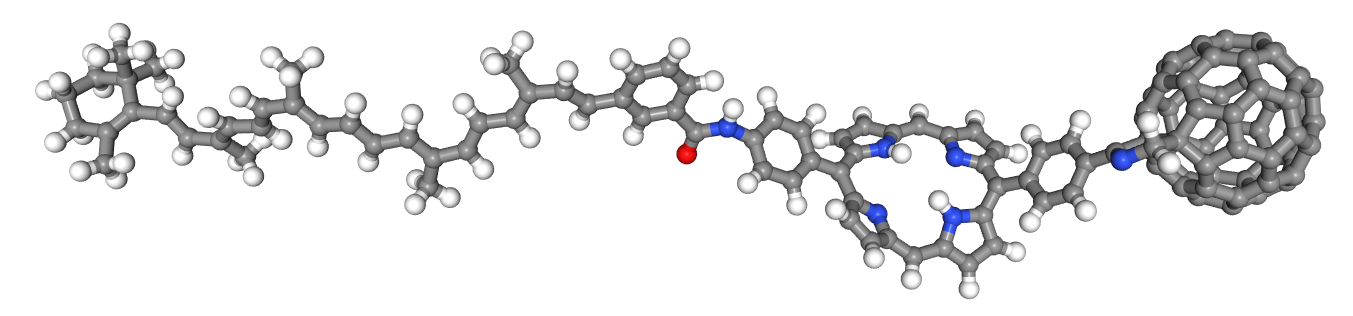
\includegraphics[width=0.4\linewidth]{projects/Gustave_Li/Docs/pics/Triad_linear.png}}
    \subfloat[Bent]{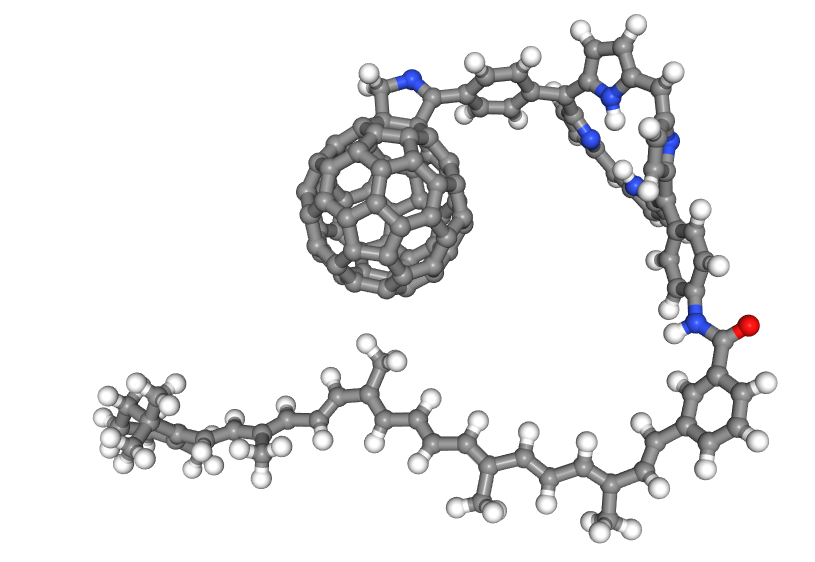
\includegraphics[width=0.3\linewidth]{projects/Gustave_Li/Docs/pics/Triad_bent.png}}
    \caption{Different conformations of \(\text{CPC}_{60}\) molecule}
    \label{fig:CPC60}
\end{figure}

Thanks to the development of computer sciences, tens of thousands of possible \(\text{CPC}_{60}\) molecules can be generated based on molecular dynamics. Considering the heavy computing load of calculation and the complexity of the \(\text{CPC}_{60}\) molecule, it is unrealistic to calculate the charge transfer rate for all the molecules. Researchers are currently working on different directions to address this issue. Brian and co-worker proposed novel formulations for calculating charge transfer rate, which reduced a maximum of 80\% of computational cost \cite{BrianDomi}. In this project, we aim to make use of machine learning to cluster the many molecules into different groups, and explore the possible machine learning pipeline that is suitable for the triad-molecule clustering scenario. By taking the cluster center as representation conformations, we expect the computational cost to decrease for a great amount while maintaining as much structural information as possible.

\section{Tools \& Platforms}

The tools and platforms used in this project are listed in Table \ref{table: tools & platforms}. Additionally, different python modules are implemented to accomplish various tasks throughout the project (see detailed information in Table \ref{table: python modules}). All the python codes and results can be found under the GitHub repository: \href{https://github.com/xiangsunlab/durf_hq/tree/master/projects/Gustave_Li}{github.com/xiangsunlab/durf\_hq/tree/master/projects/Gustave\_Li}.

\begin{table}[h!]
    \centering
    \caption{Tools and Platforms Used in the Project} 
    \begin{tabular}{l|l}
    \hline \hline
        \textbf{Tools / Platforms} & \textbf{Description} \\
        \hline
        Python & Major programming language \\
        Markdown & Light-weight note-taking language \\
        Jupyter Notebook \& Spyder & Code experiment \& module management \\
        GitHub & Project management \\
        Overleaf & Documentation \& this report \\
        NYUSH HPC & Computing resources \\
        \hline \hline
    \end{tabular}
    \label{table: tools & platforms}
\end{table}

\begin{table}[H]
    \centering
    \caption{Python Modules}
    \begin{tabular}{l|l}
    \hline \hline
        \textbf{Python modules} & \textbf{Description} \\
        \hline
        Numpy, Pandas & Data processing \\
        MDTraj\cite{MDTraj}, MDAnalysis\cite{MDAnalysis_1}\cite{MDAnalysis_2}, PyEMMA \cite{pyemma}     & Triad data reading \& analysis \\
        NGLview\cite{NGLview} & Triad molecule visualization \\
        Scikit-learn\cite{scikit-learn}, sklearn\_extra, hdbscan\cite{hdbscan} & Machine learning algorithms \\
        Matplotlib, Bokeh & Plotting \\
        \hline \hline
    \end{tabular}
    \label{table: python modules}
\end{table}

\section{Experiment Methods}

\subsection{General Workflow}
The original dataset is a molecular dynamics file containing 100,000 frames of the triad molecule. The data was first visualized to obtain basic structure and chemical features of the triad molecules. Two feature spaces were prepared for machine learning process: \textbf{a)} the xyz coordinates of each atom in the triad molecule, \textbf{b)} 8 descriptors (distances, angles, torsions) selected to represent the structure. With the feature space prepared, dimensionality reduction was applied to both spaces via different approaches and the dimensionality was reduced to 2D space for plotting and inspection conveniences. The different reduced-dimensional data were put into various clustering algorithms, which generate cluster centers (core instances) and instance labels. Quality of clustering result was evaluated with multiple criterion and some suboptimal pipelines were eliminated from the following steps. Clustering was then performed once again in the original high-dimensioanl feature space with cluster center pre-determined by the previous 2D clustering methods. Triad molecules were assigned to different clusters based on their structural similarities with core instances. High-dimensional clustering results were inspected and three machine learning methods that produces the best results were chosen.

\subsection{Descriptors}
The xyz coordinates data is the simplest feature space when it comes to describing molecular structures. However, xyz coordinates suffers from several major drawbacks: First of all, the dimension of the dataset is too high. Each triad molecule has 207 atoms with 3 coordinates for each atom, so the total dimension for each entry is 621. Such large dimension may not only take up large memory for computer to store and process the data, but also increase the risk of over fitting caused by the redundant information stored in such large dimension. Secondly, xyz coordinates are orientation sensitive. While the orientation of a single molecule has very limited effect on its chemical properties, the xyz coordinates can be very different when the molecule was translated or rotated. From this point of view, the clustering algorithm will likely to over-estimate the importance of molecular orientation and position, which gives the suboptimal result.

\subsubsection{Key Atoms \& Descriptors List}
With the aim of addressing the pitfalls of xyz data space, descriptors should be concise and not orientation-sensitive. Distances between two ends of the triad describe the overall structure of the molecule, angles and dihedrals represent the bending and twisting of each part of the molecule. RMSD with reference to the bent and linear structure displays the extent of streching and bending. The full descriptors are listed in Table \ref{table: descriptors}. Considering the three-component ( Carotenoid-Porphyrin-\(\text{C}_{60}\))  nature of the molecule and its various structures, the following atoms are chosen as key atoms and all the descriptors are computed based on them: \(\text{C}_{33}\), \(\text{C}_{21}\), \(\text{C}_{61}\), \(\text{C}_{65}\), \(\text{C}_{66}\), \(\text{C}_{69}\), \(\text{C}_{89}\), \(\text{C}_{95}\), \(\text{C}_{96}\), \(\text{C}_{128}\) and \(\text{N}_{6}\) (shown in Figure \ref{fig: key atoms}).

\begin{figure}[H]
    \centering
    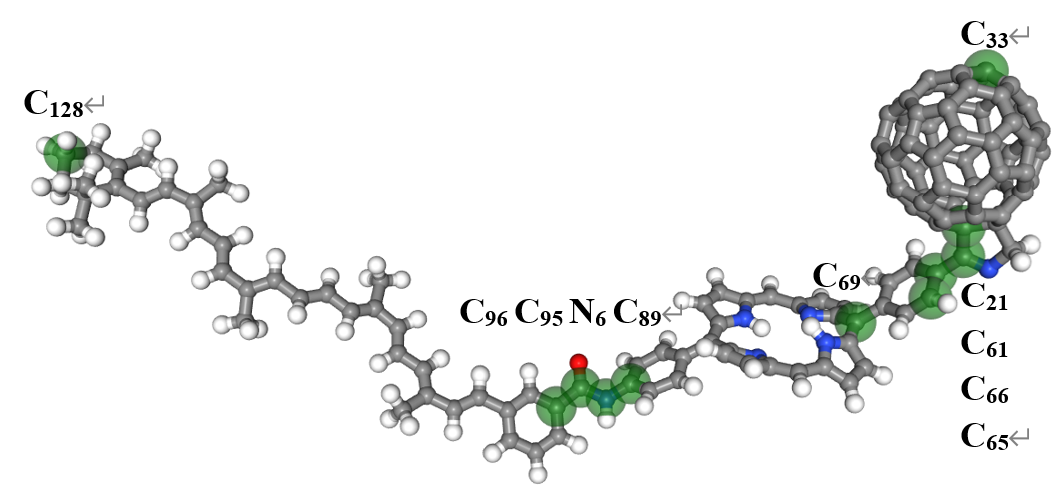
\includegraphics[width=0.75\linewidth]{projects/Gustave_Li/Docs/pics/key_atoms.png}
    \caption{Key atoms for descriptors}
    \label{fig: key atoms}
\end{figure} 

\begin{table}[H]
    \centering
    \caption{Definitions of Geometric Descriptors}
    \begin{tabular}{l|l}
    \hline \hline
       \textbf{Name}  & \textbf{Description} \\
       \hline
       EuclidianDist\_1 & The euclidian distance between \(\text{C}_{33}\) \& \(\text{C}_{128}\) \\
       Angle\_1 & The angle between atoms \(\text{C}_{33}\)-\(\text{C}_{96}\)-\(\text{C}_{128}\) \\
       Angle\_2 & The angle between atoms \(\text{C}_{33}\)-\(\text{C}_{69}\)-\(\text{C}_{96}\) \\
       Angle\_3 & The angle between atoms \(\text{C}_{69}\)-\(\text{C}_{96}\)-\(\text{C}_{128}\) \\
       Dihedral\_1 & The absolute valute of dihedral between atoms \(\text{C}_{21}\)-\(\text{C}_{61}\)-\(\text{C}_{66}\)-\(\text{C}_{65}\) \\
       Dihedral\_2 & The absolute valute of dihedral between atoms \(\text{C}_{89}\)-\(\text{N}_{6}\)-\(\text{C}_{95}\)-\(\text{C}_{96}\) \\
       RMSD\_Linear & RMSD for the conformation to the Linear triad \\
       RMSD\_Bent & RMSD for the conformation to the Bent triad \\
       \hline \hline
    \end{tabular}
    
    \label{table: descriptors}
    \vspace{1ex}
    {\noindent \justifying Note: the linear and bent conformation was determined by the overall bending angle of the triad molecule, described by the Angle\_1 descriptor. For our triad dataset, we defined the triad indexing 88213 as the linear model, which has an overall angle of \(3.10\,rad\). The bent was defined as the 29685th frame, which has an angle of \(0.36\,rad\). \par}
\end{table}

\subsection{Dimensionality Reduction}
Each of the triad molecules consist of 207 atoms, thus each molecule is represented as a data point in a 621 (\(207 \times 3\)) dimension space. In such high dimensional space, data points are far sparser than that in lower dimensional spaces, thus making it harder to find the optimal clustering result. The difficulty caused by high dimensionality is referred to as \textit{the curse of dimensionality}\cite{GeronAurelien}. Although the dimensionality was reduced to 8 by finding descriptors of the molecular structure, visualization of the 8D descriptors is still unachievable. In the face of such situation, dimensionality reduction plays its role by reducing the dimensionality of dataset significantly (to 2 or 3 for visualization) while preserving the information from original dataset\cite{GlielmoAldo}.

\subsubsection{Dimensioanlity Reduction Methods \& Hyperparameters}
Dimensionality reduction was performed on both xyz feature space and the descriptors space. Linear(PCA) and non-linear(kPCA, tSNE) dimensionality reduction methods were implemented. Hyerparameters were tuned as recorded in Table \ref{table: dimreduct}.

\begin{table}[H]
    \centering
    \caption{Dimensionality reduction method and hyperparameters}
    \begin{tabular}{p{.47\textwidth}|p{.4\textwidth}}
    \hline \hline
        \textbf{Method} & \textbf{Hyperparameters} \\
        \hline
        Principle Component Analysis (PCA) & \texttt{n\_components: 2} \\
        \hline
        kernel Principle Component Analysis (kPCA) & \texttt{n\_components: 2} \par \texttt{kernel: poly, rbf} \\
        \hline
        t-Distributed Stochastic Neighbor Embedding (t-SNE)\cite{KobakDmitry} & \texttt{n\_components: 2} \par \texttt{perplexity: 50} \par \texttt{learning\_rate: (num\_of\_data)/12} \par \texttt{init: pca} \\
        \hline \hline
    \end{tabular}
    \label{table: dimreduct}
\end{table}

\subsubsection{Dimensionality Reduction Results Inspection}
The inspection was achieved by the \texttt{pyemma.plots.plot\_density} module, which plots the dimensionality reduction results on a 2D plain and colors the data points according to the density of that region.

\subsection{Clustering}

\subsection{High-dimensioanl Clustering}

\section{Results \& Discussion}

\subsection{Dimensionality Reduction}

\subsection{Clustering}

\subsubsection{Scoring}

\subsubsection{Pairwise RMSD \& Pearson Correlation}

\subsubsection{Cluster Population}

\subsubsection{Cluster Map}

\subsection{High-dimensioanl Clustering}

\subsubsection{Cluster Population}

\subsubsection{Cluster Map}

\section{Conclusion}


\pagebreak
\bibliographystyle{unsrt}
\bibliography{references.bib}

\end{document}